\chapter{Problemen}

In dit hoofdstuk bespreken we kort de belangrijkste problemen die we ondervonden hebben tijdens de masterproef.
We zullen het hebben over randgevallen die nog niet voorzien waren door de \nwmretriever{},
de problemen op het iMinds netwerk en problemen bij het toepassen van virtualisatie op de \vwall{}.


\section{Ondersteuning voor lange OID's}
\label{probleem-lange-oids}

Een probleem waar we al redelijk vroeg op stootten, was het voorkomen van SQL-fouten bij het wegschrijven van gegevens met een lange \gls{oid} in de databank.
De grote boosdoeners hier waren de zeer lange indexen van de tabel \textit{inetCidrRouteTable} (1.3.6.1.2.1.4.24.7).

\begin{lstlisting}[language=asn.1, float=h, caption={Definitie van een inetCidrRouteEntry}, label=lst-inetCidrRouteEntry]
inetCidrRouteEntry OBJECT-TYPE 
	 SYNTAX InetCidrRouteEntry
	 MAX-ACCESS not-accessible
	 STATUS current
	 DESCRIPTION "A particular route to a particular destination, under a 
            particular policy (as reflected in the 
            inetCidrRoutePolicy object). 
 
            Dynamically created rows will survive an agent reboot. 
 
            Implementers need to be aware that if the total number 
            of elements (octets or sub-identifiers) in 
            inetCidrRouteDest, inetCidrRoutePolicy, and 
            inetCidrRouteNextHop exceeds 111, then OIDs of column 
            instances in this table will have more than 128 sub- 
            identifiers and cannot be accessed using SNMPv1, 
            SNMPv2c, or SNMPv3."
	 INDEX { inetCidrRouteDestType, inetCidrRouteDest, inetCidrRoutePfxLen, inetCidrRoutePolicy, inetCidrRouteNextHopType, inetCidrRouteNextHop } 
 	::= { inetCidrRouteTable 1  }
\end{lstlisting}

\Cref{lst-inetCidrRouteEntry} laat de definitie zien van een index uit die tabel en toont dat ze bestaat uit een samenstelling van maar liefst zes velden.
Een van die velden is een IP-adres, dat een IPv4- of een IPv6-adres kan zijn.
Zoals je weet zijn IPv6-adressen echter vrij lang, 128 bits om precies te zijn.
Een voorbeeld van een \gls{oid} uit de inetCidrRouteTable die een IPv6-adres bevat zie je in \cref{lst-lange-oids}.

\begin{lstlisting}[float=h, caption={[Tekstuele en numerieke notatie van een OID uit inetCidrRouteTable]Tekstuele en numerieke notatie van een \gls{oid} uit inetCidrRouteTable}, label=lst-lange-oids]
IP-FORWARD-MIB::inetCidrRouteIfIndex.ipv6."fe:80:00:00:00:00:00:00:0a:00:27:ff:fe:6d:bd:c5"
	.128.1.7.ipv6."00:00:00:00:00:00:00:00:00:00:00:00:00:00:00:00" = INTEGER: 1

1.3.6.1.2.1.4.24.7.1.7.2.16.254.128.0.0.0.0.0.0.10.0.39.255.254.109.189.197
	.128.1.7.2.16.0.0.0.0.0.0.0.0.0.0.0.0.0.0.0.0 = INTEGER: 1
\end{lstlisting}

Omdat de resultaattabel die de \nwmretriever{} aanmaakte slechts 55 karakters voorzag voor een \gls{oid} resulteerde dit
in SQL-fouten bij \glspl{oid} die te lang waren, zoals ook te zien is in \cref{lst-sql-error}.


\begin{lstlisting}[float=h, caption={[SQL-fout bij te lange OID]SQL-fout bij te lange \glspl{oid}}, label=lst-sql-error]
2014/02/24 14:28:54.92	Error		[21/311MB]	Failed to insert result row: 
ComfunSQLConnectionException: Error executing SQL statement: 'replace into results values(@devname,'1.3.6.1.2.1.4.34.1.5.2.16.254.128.0.0.0.0.0.0.10.0.39.255.254.109.189.197', @attrname,@value,'2014-02-24 14:28:54','OK','2014-02-24 14:28:54')' with parameters '@attrname RFC1213-MIB.ip System.String @devname debian-vm-01 System.String @value 1.3.6.1.2.1.4.32.1.5.2.2.16.254.128.0.0.0.0.0.0.0.0.0.0.0.0.0.0.64 System.String' using connectionstring 'database=snmpdb;data source=localhost;user id=xxxxx;password=xxxxx;port=3306;old syntax=yes'. ---> MySql.Data.MySqlClient.MySqlException: #22001Data too long for column 'OID' at row 1
\end{lstlisting}

De oplossing is gelukkig eenvoudig: met het vergroten van de toegelaten lengte van de \gls{oid}-kolom in de resultaattabel is het probleem opgelost.
Om dat te doen passen we simpelweg de SQL-query aan in de \nwmretriever{} die de tabel aanmaakt.
We nemen een grote marge voor de kolombreedte en vergroten ze naar 4096 karakters om toekomstige problemen te vermijden,
en omdat brede kolommen toch geen grote impact hebben.

Reeds bestaande tabellen moeten echter ofwel manueel aangepast worden om de kolom te verbreden,
ofwel kan men de tabel verwijderen en de \nwmretriever{} een nieuwe laten aanmaken indien de reeds opgeslagen resultaten verwijderd mogen worden.


\section{Ondersteuning voor de endOfMibView-exceptie}
\label{probleem-endofmibview-exceptie}

Zoals we gezien hebben in de berichtstructuur van een SNMP-bericht in \cref{snmp-berichtstructuur},
zijn er twee velden voorzien in een SNMP-bericht om aan te geven dat er zich een fout heeft voorgedaan: \textit{Error} en \textit{Error Index}.
Het eerste veld geeft met een statuscode aan of er zich een fout heeft voorgedaan, en zoja, dewelke.
Het tweede veld bevat in geval van een fout een wijzer naar het object dat de fout veroorzaakt heeft

Een van de nieuwe dingen die SNMPv2c introduceerde zijn SNMP-excepties.
Er bestaan drie zulke excepties: \textit{EndOfMibView}, \textit{NoSuchInstance} en \textit{NoSuchObject}.
Het bijzondere aan deze SNMP-excepties is dat ze toegevoegd worden aan de objectlijst (Varbind List) van een bericht
en het errorveld niet wijzigen als ze zich voordoen\cite{endOfMibView-error-status}.
Een SNMP-bericht waarin een fout is opgetreden dat aangeduidt wordt door een exceptie heeft dus nog steeds nul als waarde voor het errorveld,
wat aangeeft dat er geen fout is opgetreden.

De reden daarvoor is om het mogelijk te maken dat een exceptie zich kan voordoen samen met andere objecten die wel correct opgehaald zijn.
Herinner je dat je met GET- en GETNEXT-requests meerdere gegevens kunt ophalen,
maar dat als er zich een fout voordoet je helemaal geen gegevens terug zal krijgen met SNMPv1 (\cref{meerdere-gegevens-ophalen-met-GET-en-GETNEXT}).
Met SNMPv2c werd dit probleem dus met SNMP-excepties opgelost.

De endOfMibView-exceptie doet zich voor bij een SNMP walk wanneer er geen verdere data meer op te halen is\footnote{
	Zowel bij het gebruik van GETNEXT- en GETBULK-requests, indien gebruik gemaakt wordt van SNMPv2c of hoger.
	Bij SNMPv1 met GETNEXT-requests wordt de foutcode \textit{noSuchName} gebruikt om aan te geven dat er geen data meer is\cite{snmp-exceptions-v2c-to-v1}.
}\cite{snmp-exceptions-explained}.
Wij kwamen deze exceptie tegen bij het overlopen van een ganse SNMP-agent met de \nwmretriever{},
waarbij er op het einde natuurlijk geen gegevens meer zijn en de exceptie opgegooid wordt.

Omdat de originele versie van de \nwmretriever{} enkel gebruik maakte van GET- en GETNEXT-requests was SNMPv1 voldoende.
Bovendien is het overlopen van een ganse SNMP-agent vrij uitzonderlijk dus kwam men nooit in aanraking met deze (en de andere) excepties.
Bijgevolg werd er voor het detecteren van fouten enkel gekeken naar het erroveld en werd er dus geen rekening gehouden met excepties.

In de originele versie had dit geen gevolgen omdat excepties zich toch niet voordoen in SNMPv1.
Bij de nieuwe versie zal hier echter wel op moeten gecontroleerd worden vermits er voor bulkrequests gebruik gemaakt moet worden van SNMPv2c.

De manier om dit aan te pakken is vrij eenvoudig.
Men controleert net zoals voorheen nog steeds het errorveld, maar bij het overlopen van de objecten in het antwoordbericht
zal men ook moeten controleren of er een exceptie aanwezig is en de nodige acties ondernemen.
Bij een endOfMibView-exceptie zal men moeten de SNMP walk staken want ze is immers ten einde gelopen.


\section{''DoS-bescherming'' op intern netwerk iMinds}
\label{probleem-dos-bescherming}

\todo[inline]{Betere titel? Alhoewel de oorzaak nooit is vastgelegd...}

Een van de problemen waar we veel hinder van ondervonden hebben was een schijnbare \gls{dos} bescherming op het netwerk van iMinds.
Een \gls{dos}-aanval probeert een systeem buiten werking te stellen door bijvoorbeeld een server te overrompelen met een zo groot mogelijke hoeveelheid data.
Het gaat echter slechts om een vermoeden want de precieze oorzaak hebben we nooit kunnen vaststellen.

Het probleem doet zich voor als we een toestel bevragen in het iMinds netwerk of via het iMinds netwerk.
Dit gebeurde zowel bij het bevragen van de iMinds productieswitches als bij toestellen op de \vwall{}.
Wanneer we op korte tijd ''te veel'' verkeer genereerden --- de juiste hoeveelheid of de tijdspanne waarin dit gemeten werd hebben we niet kunnen vaststellen ---, werd alle verkeer geblokkeerd gedurende exact 20 seconden.
Het feit dat er iedere keer exact 20 seconden geen verkeer doorkon is een sterke aanwijzing dat een of andere netwerkbescherming in actie treedt.
In \cref{fig-dos-bescherming} zie je een bandbreedtegrafiek die het fenomeen toont.

\begin{figure}[h]
	\centering
	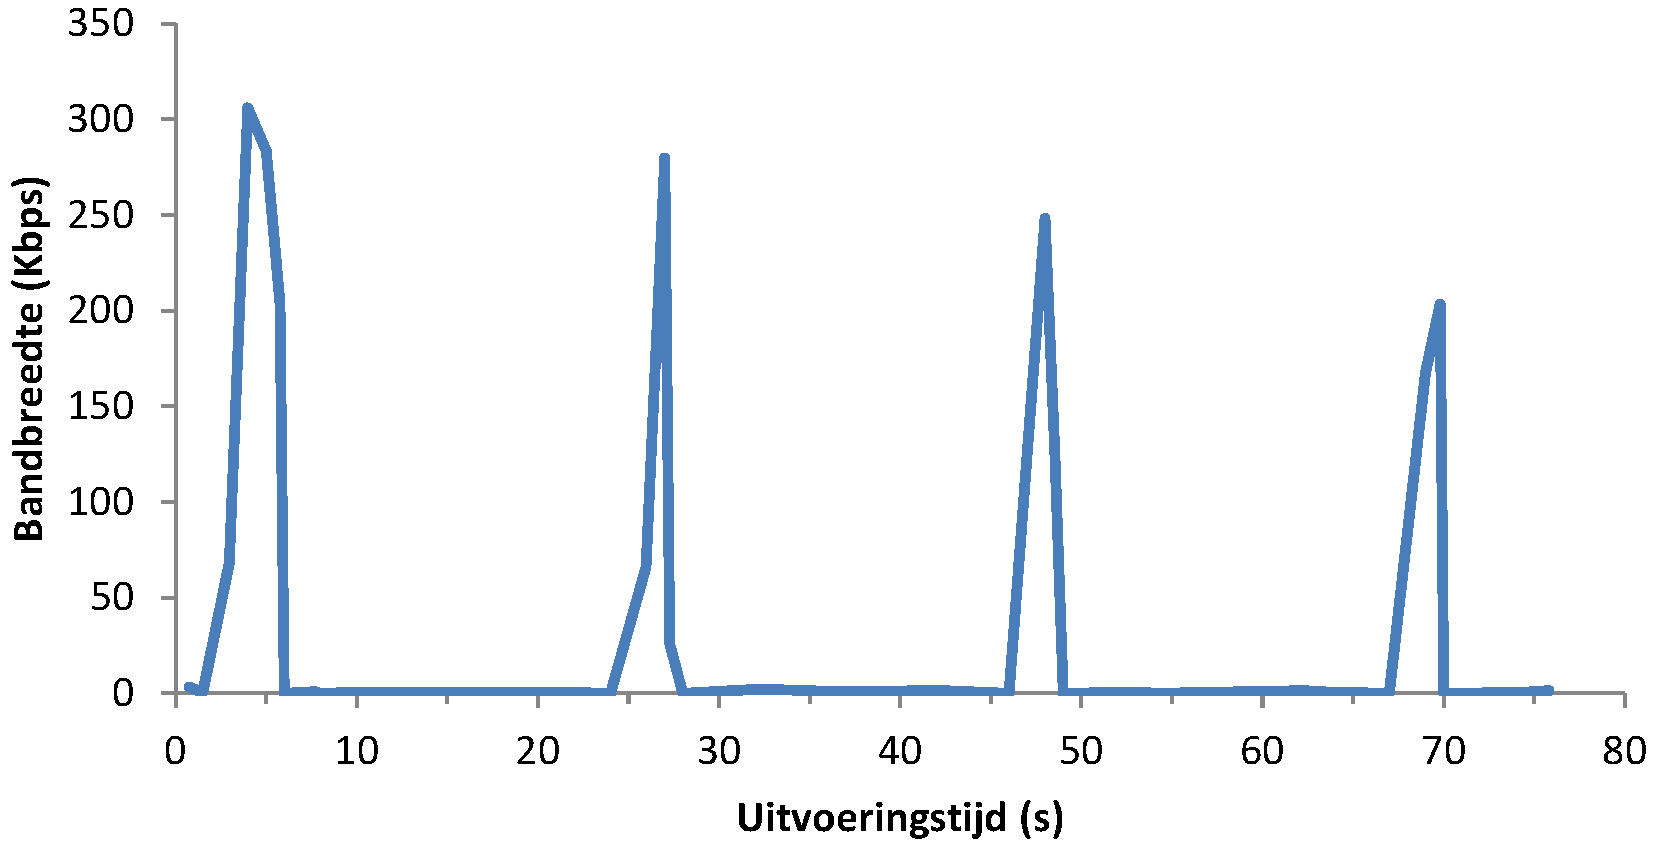
\includegraphics[scale=0.40]{figures/dos-bescherming}
	\caption{Bandbreedte tijdens het uitvoeren van tests op het iMindsnetwerk}
	\label{fig-dos-bescherming}
\end{figure}

De omstandigheden waarbij de bescherming in werking treedde konden we niet bepalen.
Er was geen bandbreedtedrempel of een limiet op het aantal pakketten per seconde die overschreden werd.
Het probleem deed zich voor bij de \nwmretriever{} maar niet bij een Net-SNMP bulkwalk,
maar dan weer wel bij onze eigen SNMP walkimplementatie die tabellen rij per rij overloopt en daarvoor Net-SNMP GETBULK-requests gebruikt.

We zijn ook bij de netwerkbeheerders van iMinds ten rade gegaan maar zij hadden geen weet van wat er verantwoordelijk zou kunnen zijn hiervoor.

Bij de kleinschalige tests die gebruik maakten van de productieswitches konden we wel nog resultaten bekomen als we zeer weinig iteraties uitvoerden.
Op die manier konden we toch nog een idee krijgen of de tests op de virtuele machines een realistisch beeld gaven van de werkelijkheid.

Bij de grootschalige tests was het probleem eenvoudig opgelost door simpelweg ook het toestel waarop de \nwmretriever{} draaide ook in de \vwall{} te plaatsen.
Door een directe verbinding te leggen tussen de retriever en de toestellen ging het verkeer niet meer over het iMinds netwerk maar bleef het geïsoleerd in de \vwall{} waarop geen netwerkbeperkingen van toepassing zijn.


\section{Virtualisatie op de Virtual Wall}
\label{probleem-virtualisatie-vwall}

Een netwerkopstelling op de Virtual Wall wordt geconfigureerd aan de hand van een script die de \textit{NS-file} genoemd wordt en
waarin men de machines en de netwerkverbindingen definieert.

Virtualisatie wordt ondersteund op de \vwall{} maar is nog volop in ontwikkeling volgens de documentatie.
Men kan hierbij gebruik maken van OpenVZ of Xen\cite{vwall-openvz, vwall-xen}.
Om hiervan gebruik te maken volstaat het om andere parameters mee te geven met de gedefinieerde machines in de NS-file,
zodat aangeven wordt dat het om virtuele machines gaat.
De \vwall{} zorgt er dan voor dat de nodige hostmachines voorzien worden en de gevraagde toestellen gevirtualiseerd worden.

De problemen die wij ondervonden hadden te maken met compatibiliteitsproblemen met de netwerkencapsulatiemethoden.
Er zijn twee zulke encapsulatiemethoden: \textit{veth-ne} en \textit{vlan}.
Standaard wordt de eerste gebruikt maar men kan er ook voor kiezen om de tweede te gebruiken.
Documentatie hierover is echter zo goed als niet te vinden.

Om meerdere toestellen allemaal met elkaar te verbinden definieert men in de NS-file een LAN-netwerk en voegt men daar alle toestellen aan toe.
In de praktijk wordt dat dan vertaald door een switch waar alle toestellen aanhangen.
Het probleem is dat als men de standaardencapsulatie gebruikt, de virtuele machines daar niet mee overweg kunnen.
De foutmelding die gegeven wordt bij het opzetten van de netwerkopstelling ziet er zo uit:

\begin{lstlisting}
Encapsulation not supported on big-lan since at least one of the nodes in big-lan does not support 'veth-ne' link emulation
\end{lstlisting}

Hierbij werd het LAN-netwerk \textit{'big-lan'} genoemd.
Als men de vlan-encapsulatiemethode gebruikt, kunnen de niet-gevirtualiseerde machines daar op hun beurt niet mee overweg.
Het komt er dus op neer dat we alle virtuele machines wel met elkaar kunnen verbinden maar niet met fysieke machines,
ondanks dat dit volgens de documentatie wel mogelijk zou moeten zijn, zelfs zonder de encapsulatiemethode te wijzigen\cite{vwall-openvz}.

De oplossing die wij dan uiteindelijk hebben gebruikt, was om zelf de virtualisatie te configureren met behulp van \gls{lxc} (zie \cref{lxc}).


\todo[inline,caption={}]{

\begin{itemize}

	\item Kolombreedte OID's (en andere? Hostnaam?) te klein
	\item endOfMibView exceptie niet ondersteund door SNMP Data Retriever \\
		Zie pg. 7, verslag week 9-10
	\item Grootschalige testopstelling op de Virtual Wall \\
		Probleem met de virtualisatie (beta achtige feature, werkt in de praktijk niet zo goed)
		Problemen met netwerkopstelling/adapters voor virtuele nodes
	
\end{itemize}

Niet opgelost/niet belangrijk:

\begin{itemize}

	\item DDOS-bescherming bij iMinds
	\item Permissieproblemen met snmpd.	$ \rightarrow $ IP range beperking~
	\item Omdat mijn reactietijden.pl script maar een commando uitvoert, hebben we voor het benchmarken van bulkrequests die manueel opgesteld worden een ander script nodig.
	Ik heb me hiervoor gebaseerd op m'n benchmarking script voor Windows die zelf de tijden meet (omdat ik de /usr/bin/time van Linux niet heb in Windows).
	Deze maakt gebruik van een CPAN module. Om zeker te zijn dat er geen grote verschillen tussen de timing-methoden zitten, heb ik nog een derde manier geprobeerd.
	Ik maak gebruik van HiRes time en hou start- en eindtijd bij en geef het verschil terug. De drie timingmethoden komen dicht genoeg bij elkaar in de buurt om te concluderen
	dat er geen timingverschillen optreden bij het gebruik van verschillende timingmethoden en ik dus de tijden kan vergelijken. \\
	Zie ook meerderekolommen - Vergelijk timings.pl en Verschillen in benchmark timings.txt.
	\item Totaal aantal objecten dat een agent aanbiedt.
	\item Gaten in tabellen, zie random notes.txt
	\item Problemen met verouderde softwarepakketten op Debian
	
\end{itemize}

}